\chapter{Feedback}\label{c:feedback}
\section{Uses of Feedback}
\begin{itemize}
\item disturbance rejection
\item parameter sensitivity
\item command tracking
\end{itemize}
\section{Anatomy of Feedback Control}

\begin{figure}[hbt]
\centering
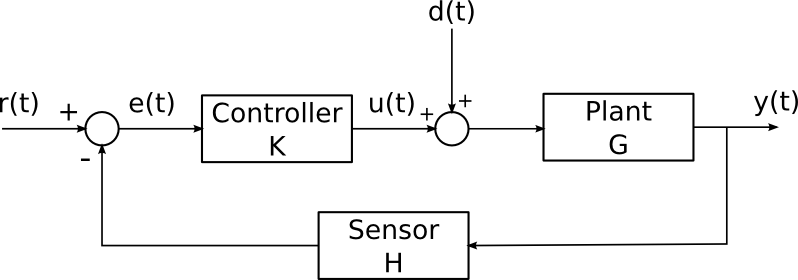
\includegraphics[width=\FigWidth\textwidth]{feedback.png}
\caption{Canonical feedback control system block diagram.}
\label{f:fdbk}
\end{figure}

\begin{itemize}
\item process
\item disturbance
\item actuator
\item plant 
\item controller
\item sensor
\end{itemize}


\section{PID Control}

\begin{equation}\label{e:pid}
u(t) = K_p e(t) + K_i \int_0^te(\tau) \mathrm{d}\tau + K_d \frac{\mathrm{d}}{\mathrm{d}t}e(t)
\end{equation}

\section{Assessing Stability}
Conceptually, a dynamic system is considered stable if the outputs of the system remain finite in response to finite inputs.  A slightly more restrictive definition is known as bounded-input bounded-output (BIBO) stability.  A system is BIBO stable if the output is less than some value, the bound, in response to an input that is bounded.  In either case, the output of an unstable system will grow to very large values---certainly something to avoid when designing control systems for robots.

As an example consider our first-order model of a car (\ref{e:car}) repeated here as
\[
m\left(\dot{v}(t)\right) + b(v(t)) = f(t)
\]
and the solution for the step response with zero initial velocity
\[
v(t) = F/b \left(1-e^{-t/(m/b)} \right).
\]
Consider the same model, but the value for the damping parameter $b$ is negative.  Let's say $b=-1$, but really any negative number will do.  Now the solution to the differential equations is of the form
\[
v(t) = F \left(1-e^{t/(m)} \right).
\]
The velocity grows exponentially with time towards infinity!

\begin{ex}
Show that a first order system with {\bf positive} feedback can produce an unstable response.
\end{ex}

\section{Assessing Performance}



\section{Exercises}
\begin{ex}
Using our first order car model with the parameters given in Exercise~\ref{ex:carstep} design a closed-loop feedback controller, a ``cruise control'', that will regulate the car's velocity.  Here are the requirements for your controller:
\begin{itemize}
\item Minimize the rise time, overshoot and stead-state error
\item The control force (car input) cannot exceed \unit[15,000]{N}.
\end{itemize}

Our test scenario is a step change in the speed command ($r(t)$) from 0 to \unit[60]{mph}. Produce a graph of the speed of the car starting from stationary with a constant reference command of \unit[60]{mph}.  Also produce a graph of the control force for the same test.

Submit a short description of your control algorithm that documents the algorithm in equations and full sentences.  Report the rise time, percent overshoot and steady-state error for your design in the test scenario (0 to \unit[60]{mph}
\end{ex}

\begin{ex}
In the previous exercise you generated a control algorithm to regulate the speed of ``car''.  In this exercise you will generate a control algorithm to regulate the position of your ``car''.

First you will need a model.  Write a continuous time second-order differential equation to describe the position ($x(t)$) of the car.  Write a program to solve this model using the Euler method.

Once you have a working model, design a control algorithm to regulate the position of the car.   Here are the requirements for your controller:
\begin{itemize}
\item Minimize the rise time, overshoot and stead-state error
\item The control force (car input) cannot exceed \unit[15,000]{N}.
\end{itemize}

Our test scenario is a step change in the position command ($r(t)$) from 0 to \unit[100]{m}. Produce a graph of the speed of the car starting from stationary with a constant reference command of \unit[100]{m}.  Also produce a graph of the control force for the same test.

Submit a short description of your control algorithm that documents the algorithm in equations and full sentences.  Report the rise time, percent overshoot and steady-state error for your design in the test scenario (0 to \unit[100]{m}
\end{ex}
